% !TeX encoding = UTF-8

\chapter{IMPLEMENTAÇÃO DAS TÉCNICAS}\label{ch:implementacao}
Este capítulo tem como objetivo, apresentar de forma mais detalhada todo o processo de desenvolvimento realizado no presente trabalho, com o intuito de alcançar os objetivos especificados no Capítulo 1.

\section{REALIZAÇÃO DA COLETA DE DADOS}
Tendo em vista as ferramentas necessárias para realizar a coleta das séries temporais que serão utilizadas para o treinamento e testes da RNA, foi desenvolvido um método de automatização de aquisição das ações que serão utilizadas para a análise.

Inicialmente, foi criada uma interface em Python que contém a assinatura do método que as empresas deverão implementar. Após isso, foram criadas as classes para as respectivas empresas, definidas no seção 4.2. Para exemplificar de forma mais intuituva, o código 3 demonstra a implementação do atual procedimento. 
\codigoPython\
\lstinputlisting[label=cod:exempla-coleta, caption=Implementação da interface Empresa em Python]{src/empresa.py}

Analisando o código acima, pode-se observar o desenvolvimento da interface "Empresa"\, e da classe "Apple", que implementa esta interface através da parâmetro (Empresa) em sua definição. Também é possível observar na classe Apple a implementação do método construtor "\_\_init\_\_"\, que contém seu respectivo nome e código, necessário para realizar a busca. O método "executa\_busca", por sua vez, faz uma chamada ao objeto que realizará a coleta das respectivas ações, passando seus parâmetros como valor. O código 4 ilustra a implementação do objeto de busca.
\codigoPython\
\lstinputlisting[label=cod:exemplo-crawler, caption=Implementação do objeto Crawler que realiza a busca das ações]{src/crawler.py}

O código acima utiliza a biblioteca pandas para realizar a coleta das ações. Pode-se observar que o método construtor "\_\_init\_\_"\, recebe o nome e o código da empresa que faz a chamada de sua instância. Também é possível analisar o método "executa\_busca"\, implementado, que realiza a chamada da função "web.DataReader"\,
passando quatro parâmetros, sendo eles:
\begin{enumerate}
\item Código da empresa;
\item API que será realizada a busca;
\item Data de inicial da coleta;
\item Data final da coleta.
\end{enumerate}

Após a realização da requisição, a API retornará um arquivo com as ações entre as respectivas datas, no formato especificado na seção 4.4.2. Este procedimento foi realizado para todas as empresas que serão analisadas neste trabalho. A seguir, serão analisadas as séries específicas de cada empresa, através de seus valores diários de abertura.

Iniciando por ordem alfabética, as ações da Amazon, coletadas entre o período de 09/04/2001 a 31/08/2017 contém os valores mais altos dentre as empresas estudadas. No período coletado, seu valor de abertura apresentou um mínimo de 5,91 e um máximo de 1069,55 dólares Americanos (USD), evidenciando seu crescimento e valorização. A Figura 13 representa o comportamento desta série.
\begin{figure}[h]
	\centering
	\centerline{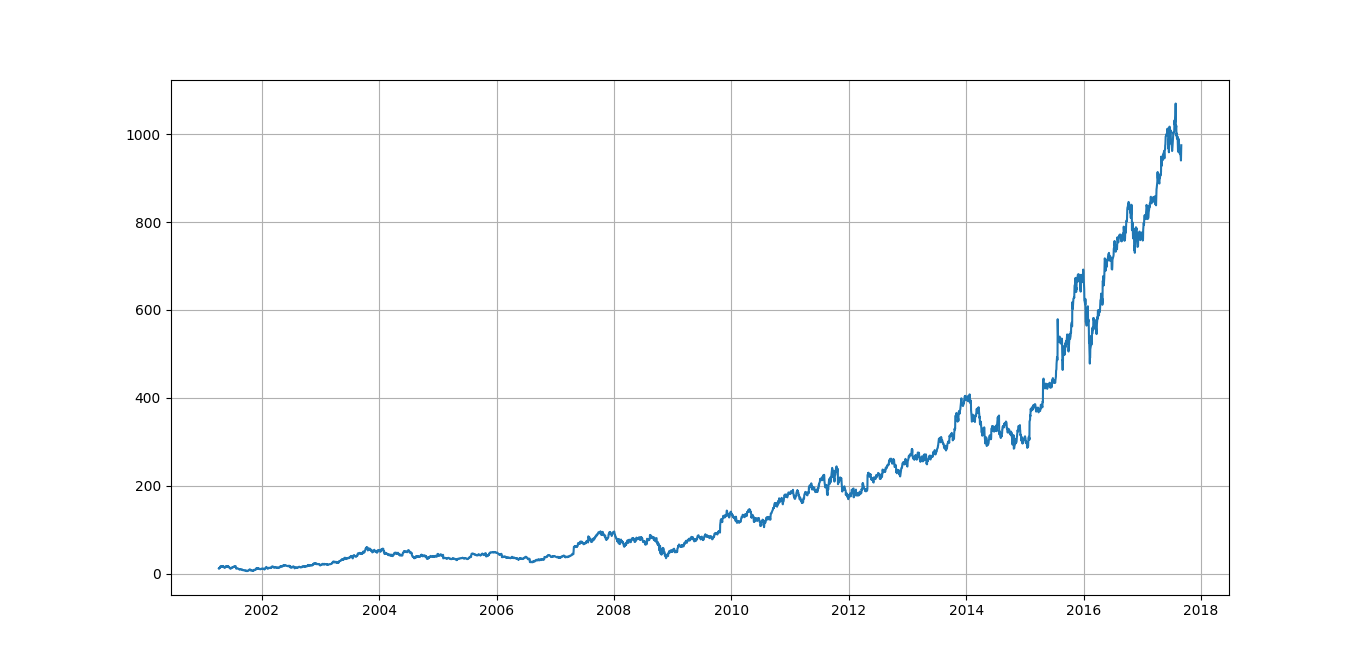
\includegraphics[scale=4]{amazon_coletado}}
	\caption{Valores de abertura das ações da Amazon}
	\fonte{Elaborado pelo autor}
	\label{exec-amazon-coleta}
\end{figure}